All of the protocols were implemented in Java 6 on a server (3GHz AMD processor, 6GB of RAM) running Ubuntu 12.04. These
benchmarks measured latency, the amount of work each device would have to do in the group excluding communication.
In each test, 2048-bit primes $p$ are used; the values for SPEKE+ and J-PAKE+ were used as in Hao et. al.~\cite{HaYiChSh15}.
Values for PPK+ were taken from J-PAKE+, and values for Dragonfly+ were taken from the NIST cryptographic toolkit~\cite{NIST}.
\\

For groups sizes from 3 to 20 participants, we measure the latency of computation at each round of the protocol. The measurement
was done by repeating the same experiment 100 times and taking the average values. The results are summarized in Figure \ref{fig:results}.

\begin{figure}[h]
    \centering
    \begin{subfigure}[b]{0.5\textwidth}
        \centering
        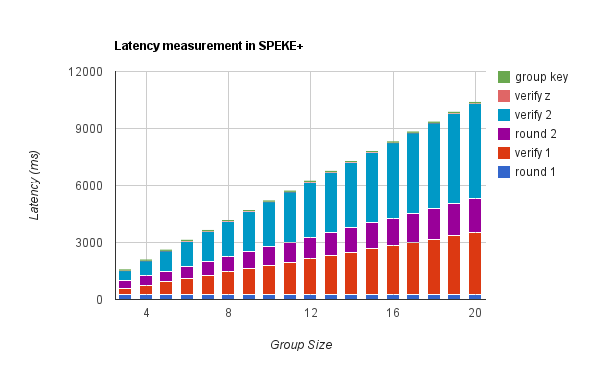
\includegraphics[width=\textwidth]{benchmark/speke.png}
        \caption{SPEKE+ latency results.}
        \label{fig:speke_results}
    \end{subfigure}
    ~
    \begin{subfigure}[b]{0.5\textwidth}
        \centering
        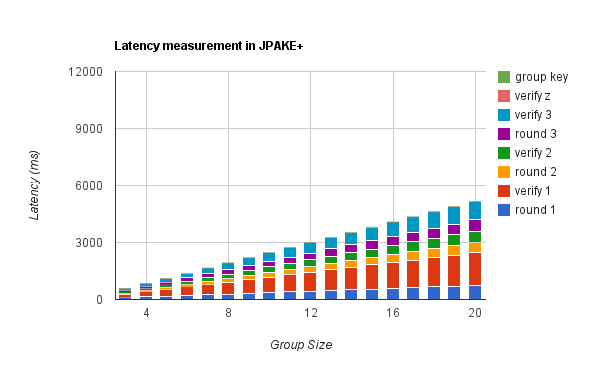
\includegraphics[width=\textwidth]{benchmark/scale_jpake.png}
        \caption{JPAKE+ latency results.}
        \label{fig:jpake_results}
    \end{subfigure}
    \begin{subfigure}[b]{0.5\textwidth}
        \centering
        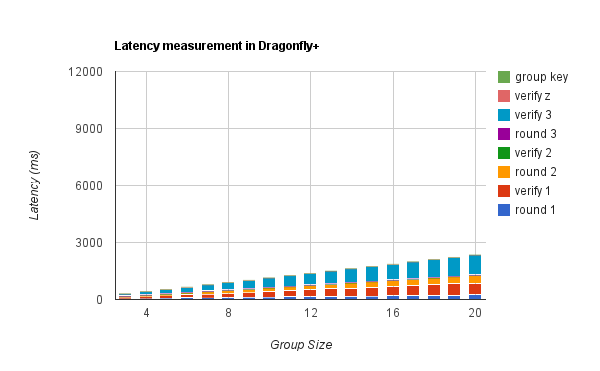
\includegraphics[width=\textwidth]{benchmark/scale_dragon.png}
        \caption{Dragonfly+ latency results.}
        \label{fig:dragon_results}
    \end{subfigure}
    ~
    \begin{subfigure}[b]{0.5\textwidth}
        \centering
        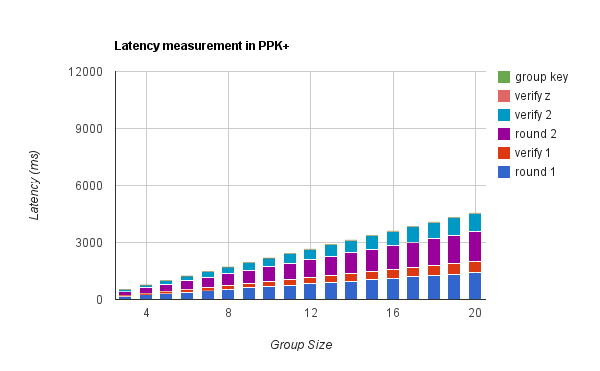
\includegraphics[width=\textwidth]{benchmark/scale_ppk.png}
        \caption{PPK+ latency results.}
        \label{fig:ppk_results}
    \end{subfigure}
    \caption{Latency measurement results for the GPAKE extensions of each of the PAKE protocols.}
    \label{fig:results}
\end{figure}

%\begin{center}
%    \begin{figure}[h]
%        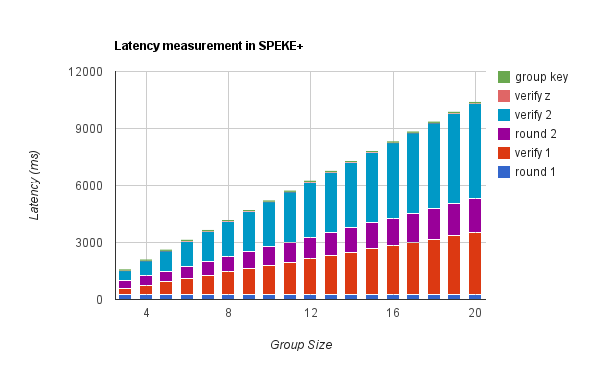
\includegraphics[scale=0.5]{benchmark/speke.png}
%        \caption{SPEKE+ latency results.}
%        \label{fig:speke_results}
%    \end{figure}
%    \begin{figure}[h]
%        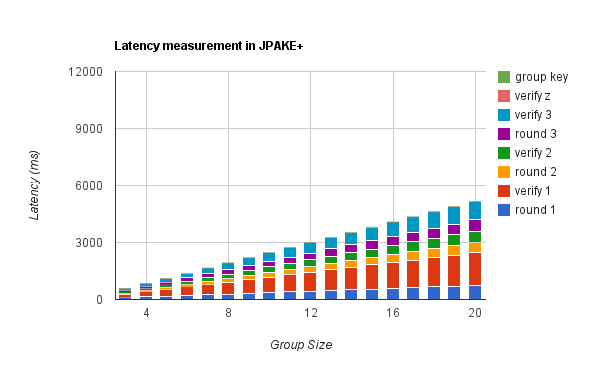
\includegraphics[scale=0.5]{benchmark/scale_jpake.png}
%        \caption{JPAKE+ latency results.}
%        \label{fig:jpake_results}
%   \end{figure}
%    \begin{figure}[h]
%        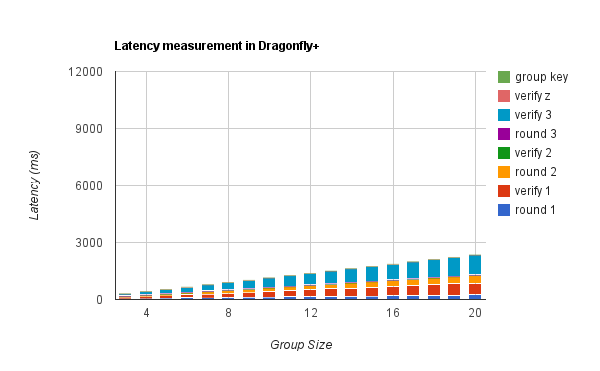
\includegraphics[scale=0.5]{benchmark/scale_dragon.png}
%        \caption{Dragonfly+ latency results.}
%        \label{fig:dragon_results}
%    \end{figure}
%    \begin{figure}[h]
%        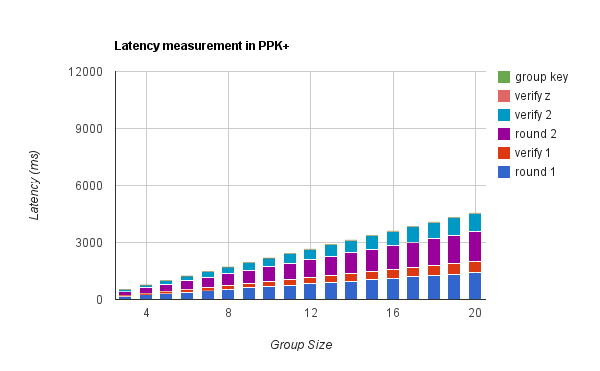
\includegraphics[scale=0.5]{benchmark/scale_ppk.png}
%        \caption{PPK+ latency results.}
%        \label{fig:ppk_results}
%    \end{figure}
%\end{center}

As shown in Figure \ref{fig:results}, the total latency for each member increases linearly with the size of group, regardless of the protocol.  To begin, we see that SPEKE+ is the slowest protocol, due in part to its need of a `safe' prime of the form $q = 2p-1$.  This means that when $p$ is a 2048-bit prime, $q$ is a 2047-bit prime, which is much larger than what is needed for the other algorithms (typically, with primes in the hundreds of digits the assumptions needed for our PAKE security are considered to be safe).  Although Dragonfly+ is considerably the fastest GPAKE here, it uses 3 rounds of communication -- compared to only 2 for J-PAKE+ and PPK+ -- and the underlying PAKE protocol does not have a security proof.  The PPK+ protocol which we constructed, on the other hand, is built from a two party PAKE with a stronger security proof than J-PAKE and runs faster than J-PAKE+.  Thus, this seems like a good candidate for future research.
\\

We now conclude by summing up the work presented here and giving some directions for future work in this area.

